\chapter{Question 7 - Particle Filtering}
\assignment{
  \begin{enumerate}
    \item What is the differences between PF and EKF/UKF from a methodology point of view?
    \item What is the differences between PF and EKF/UKF from a application/practice point of view?
  \end{enumerate}
}

\section{Particle filter} % (fold)
\label{sec:particle_filter}
The particle filter is good at starting without known states.

\textbf{N = 0, before any measurements} \\
The states could be anywhere in the possible sets \\
% \begin{figure}
%         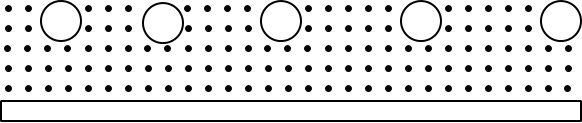
\includegraphics[width=2.5cm]{n0.png}
% \end{figure}
\textbf{N = 1, first measurements} \\
The measurements make some states very unlikely, there are still several possible sets. \\
The states then change , a controller reacts to the states. \\
\textbf{N = 2, second measurements} \\
New measurements are made, and the particle cloud is updated based on previous cloud \\


% section particle_filter (end)

\section{Extended Kalman Filter} % (fold)
\label{sec:extended_kalman_filter}
Measurement update (estimation, based on model, measurements and inputs)
\begin{equation}
        \begin{split}
              \vect{\hat{y}}_{k \vert k-1} &= h(\vect{\hat{x}}_{k \vert k-1},\vect{u}_k) \\
              \vect{\tilde{y}}_{k \vert k-1} &= \vect{y}_{k} - \vect{\hat{y}}_{k \vert k-1} \\
              \matt{K}_k &= \matt{P}_{k \vert k-1} \g \matt{H}_{k} \transp \g (\matt{H}_k \g \matt{P}_{k \vert k-1} \g \matt{H}_{k} \transp + \matt{R}_k )^{-1}  \\
              \vect{\hat{x}}_{k \vert k} &= \vect{\hat{x}}_{k \vert k-1} + \matt{K}_k \g \vect{\tilde{y}}_{k \vert k-1} \\
              \matt{P}_{k \vert k} &= (\matt{I} - \matt{K}_k \g \matt{H}_k) \g \matt{P}_{k \vert k-1} \g (\matt{I} - \matt{K}_k \g \matt{H}_k) \transp + \matt{K}_k \g \matt{R}_k \g \matt{K}_k \transp
        \end{split}
\end{equation}
Time update (Prediction)
\begin{equation}
\begin{split}
        \vect{\hat{x}}_{k+1 \vert k} &= f(\vect{\hat{x}}_{k \vert k}, \vect{u}_k) \\
        \matt{P}_{k +1 \vert k} &= \matt{F}_k \g \matt{P}_{k \vert k} \g \matt{F}_{k}\transp + \matt{Q}_k
\end{split}
\end{equation}

% section extended_kalman_filter (end)

\section{Unscented Kalman Filter} % (fold)
\label{sec:unscented_kalman_filter}
Measurement update 
\begin{equation}
        \begin{split}
                \begin{bmatrix}
                \vect{\hat{y}}_{k \vert k-1} \\[2mm]
                \matt{Cov}(\vect{\tilde{y}}_{k \vert k-1}, \vect{\tilde{x}}_{k \vert k-1}) \\[2mm]
                \matt{C}_{k}^{h}
                \end{bmatrix} &= U(h, \vect{\hat{x}}_{k \vert k-1}, \matt{P}_{k \vert k -1}) \\
                \matt{Cov}(\vect{\tilde{y}}_{k \vert k-1}) &= \matt{C}_{k}^{h} + \matt{R}_k \\
                \matt{Cov}(\vect{\tilde{x}}_{k \vert k-1},\vect{\tilde{y}}_{k \vert k-1}) &= \matt{Cov}(\vect{\tilde{y}}_{k \vert k-1},\vect{\tilde{x}}_{k \vert k-1})\transp \\
                \vect{\tilde{y}}_{k \vert k-1} &= \vect{y}_k - \vect{\hat{y}}_{k \vert k-1} \\
                \matt{K}_k &= \matt{Cov}(\vect{\tilde{x}}_{k \vert k-1},\vect{\tilde{y}}_{k \vert k-1})\matt{Cov}(\vect{\tilde{y}}_{k \vert k-1})^{-1} \\
                \vect{\hat{x}}_{k \vert k} &= \vect{\hat{x}}_{k \vert k-1} + \matt{K}_k \g \vect{\hat{y}}_{k \vert k-1} \\
                \matt{P}_{k \vert k} &= \matt{P}_{k \vert k-1} - \matt{K} \g \matt{Cov}(\vect{\tilde{y}}_{k \vert k-1},\vect{\tilde{x}}_{k \vert k-1})
        \end{split}
\end{equation}

Time update (prediction)
\begin{equation}
        \begin{split}
                \begin{bmatrix}
                \vect{\hat{x}}_{k+1 \vert k} \\[2mm]
                \matt{X} \\[2mm]
                \matt{C}_{k}^{f}
                \end{bmatrix} &= U(f,\vect{\hat{x}}_{k \vert k}, \matt{P}_{k \vert k}) \\
                \matt{P}_{k + 1 \vert k} &= \matt{Cov}(\vect{\tilde{x}}_{k+1 \vert k}) = \matt{C}_{k}^{f} + \matt{Q}_k
        \end{split}
\end{equation}

% section unscented_kalman_filter (end)